\documentclass[a4paper, 12pt]{article} % тип документа

%%%Библиотеки
	%\usepackage[warn]{mathtext}	
	\usepackage[T2A]{fontenc}   %Кодировка
	\usepackage[utf8]{inputenc} %Кодировка исходного текста
	\usepackage[english, russian]{babel} %Локализация и переносы
	\usepackage{caption}
	\usepackage{listings}
	\usepackage{amsmath, amsfonts, amssymb, amsthm, mathtools}
	\usepackage[warn]{mathtext}
	\usepackage[mathscr]{eucal}
	\usepackage{wasysym}
	\usepackage{graphicx} %Вставка картинок правильная
	\DeclareGraphicsExtensions{.pdf,.png,.jpg}
	\graphicspath{ {images/} }
	
	\setlength{\parskip}{0.5cm}
	
	\usepackage{pgfplots}
	\usepackage{indentfirst}
	\usepackage{float}    %Плавающие картинки
	\usepackage{wrapfig}  %Обтекание фигур (таблиц, картинок и прочего)
	\usepackage{fancyhdr} %Загрузим пакет
	\usepackage{lscape}
	\usepackage{xcolor}
	\usepackage[normalem]{ulem}
	\usepackage{wasysym}
	
	\usepackage{titlesec}
	\titlelabel{\thetitle.\quad}

	\usepackage{hyperref}
	\newenvironment{comment}{}{}

%%%Конец библиотек

%%%Настройка ссылок
	\hypersetup
	{
		colorlinks = true,
		linkcolor  = blue,
		filecolor  = magenta,
		urlcolor   = blue
	}
%%%Конец настройки ссылок


%%%Настройка колонтитулы
	\pagestyle{fancy}
	\fancyhead{}
	\fancyhead[L]{2.4.1}
	\fancyhead[R]{Старченко Иван, группа Б01-005}
	\fancyfoot[C]{\thepage}
%%%конец настройки колонтитулы

\begin{document}

%\maketitle
%\thispagestyle{empty}

%\newpage
\setcounter{page}{1}



\begin{center}
  \LARGE{Лабораторная работа 3.3.4}\\[0.2cm]
  \LARGE{Эффект Холла в полупроводниках.}\\[0.2cm]
  \large{10 сентября 2021 г.}\\[0.2cm]
  \large{Старченко Иван Александрович}\\[0.2cm]
\end{center}

\textbf{Цель работы:} \\
Измерение подвижности и концентрации носителей заряда в полупроводниках.

\textbf{В работе используются:} \\
Электромагнит с источником питания, батарейка, амперметр, реостат, цифровой вольтметр, милливеберметр, образцы легированного германия.
 


	\section{Экспериментальная установка.}
	Схема экспериментальной установки показана на рис. 2.
	
	\begin{figure}[h!]
		\centering
		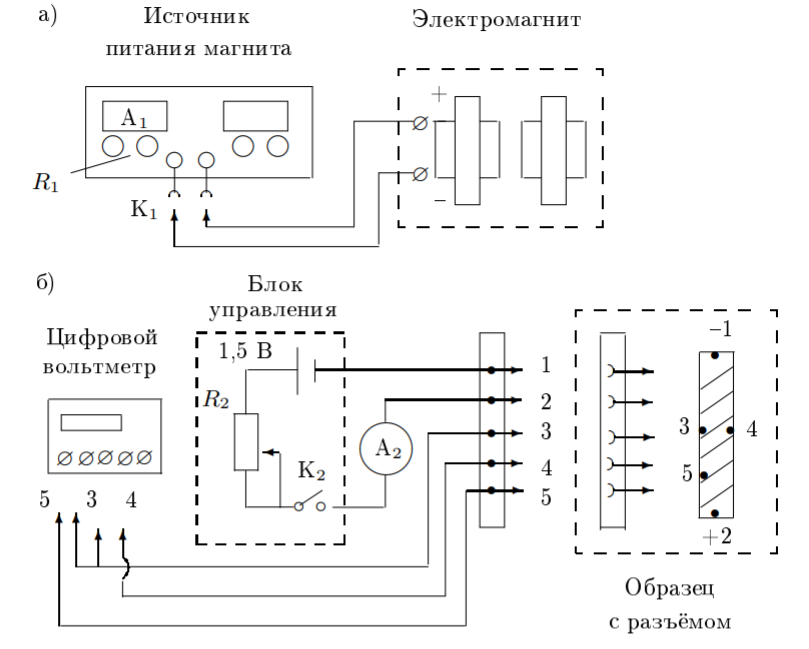
\includegraphics[width=\linewidth]{1}
		\caption{Схема установки для исследования эффекта Холла в полупроводниках}
		\label{fig:Holl2}
	\end{figure}
  
  	В зазоре электромагнита (рис. 1а) создаётся постоянное магнитное поле, величину которого можно менять с помощью регуляторов источника питания. Ток измеряется амперметром источника питания $A_{1}$. Разъем $K_{1}$ позволяет менять направление тока в обмотках электромагнита.
  
  	Образец из легированного германия, смонтированный в специальном держателе (рис. 1б), подключается к батарее. При замыкании ключа $K_{2}$ вдоль длинной стороны образца течет ток, величина которого регулируется реостатом $R$ и измеряется миллиамперметром $А_{2}$.
  	
  	В образце с током, помещённом в зазор электромагнита, между контактами 3 и 4 возникает разность потенциалов $U_{34}$, которая измеряется с помощью цифрового вольтметра.
  	
  	Контакты 3 и 4 вследствие неточности подпайки не всегда лежат на одной
  	эквипотенциали, и тогда напряжение между ними связано не только с эффектом
  	Холла, но и с омическим падением напряжения, вызванным протеканием основного тока через образец.
  	
  	Измеряемая разность потенциалов при одном направлении
  	магнитного поля равна сумме ЭДС Холла и омического падения напряжения, а
  	при другом  их разности. В этом случае ЭДС Холла $\mathscr{E}_{X}$ может быть определена как половина алгебраической разности показаний вольтметра, полученных для
  	двух противоположных направлений магнитного поля в зазоре.
  	
  	Можно исключить влияние омического падения напряжения иначе, если при каждом токе через образец измерять напряжение между точками 3 и 4 в отсутствие магнитного поля. При фиксированном токе через образец это дополнительное к ЭДС Холла напряжение $U_{0}$ остается неизменным. От него следует (с учетом
  	знака) отсчитывать величину ЭДС Холла: 
  	
  	$$\mathscr{E}_{X} = U_{34} \pm U_{0}$$. 
  	
  	При таком способе измерения нет необходимости проводить повторные измерения с противоположным направлением магнитного поля.
  	
  	
  	По знаку $\mathscr{E}_{X}$ можно определить характер проводимости - электронный или дырочный. Для этого необходимо знать направление тока в образце и направление
  	магнитного поля.
  	
  	Измерив ток $I$ в образце и напряжение $U_{35}$ между контактами 3 и 5 в отсутствие магнитного поля, можно, зная параметры образца, рассчитать проводимость материала образца по формуле:
  	
  \begin{equation}\label{sigma}
  	\sigma=\dfrac{I\cdot L_{35}}{U_{35}\cdot a\cdot l}
  \end{equation}
  	
  	где $L_{35}$ - расстояние между контактами 3 и 5, $a$ - толщина образца, $l$ - его ширина.


\section{{Ход работы}}






\section{{Апроксимация полученных данных}}


\section{{Вывод}}


Мы изучили явление эффекта Холла в полупроводниках, измерили для нашего образца (Германий) такие величины как постоянная Холла, концентрацию электронов, удельную проводимость и подвижность электронов.



\section{{Список используемой литературы}}

$\bullet$ \href{https://vk.com/doc-139677307_612194888}{Никулин М.Г. Лабораторный практикум по общей физике. Электричество и магнетизм}\\

$\bullet$ \href{https://mipt.ru/education/chair/physics/S_III/lab_el.php}{Описание лабораторных работ на кафедре общей физики МФТИ}

$\bullet$ \href{https://vk.com/doc-139677307_612194961}{П.В. Попов, А.А. Нозик. Обработка результатов учебного эксперимента}


 













 




\end{document}